%% This document created by Scientific Word (R) Version 2.5
%% Starting shell: mathart1


\documentclass[a4paper]{article}
%\usepackage{RR}
%\usepackage[latin1]{inputenc}
\usepackage{epsfig,float}
\usepackage{amssymb,amsmath,graphics,showkeys}
\newtheorem{theorem}{Theorem}[section]
\newtheorem{definition}{Definition}[section]
\newtheorem{proposition}{Proposition}[section]
\newtheorem{Assumption}{Assumption}
\newtheorem{lemma}{Lemma}[section]
\newtheorem{Corollary}{Corollary}[section]
\newtheorem{remark}{Remark}[section]
\newtheorem{example}{Example}[section]
\textheight=624pt \topmargin=28pt \textwidth=15,5cm
\oddsidemargin=1cm \evensidemargin=-.5cm

\author{Vlad Bally \and Emmanuel Temam}

\title{Empirical semi-groups and calibration}
\begin{document}
\maketitle
\begin{abstract}
We present a probabilistic method to calibrate a Markovian model
to a finite set of observed options prices. In this frame, the aim
of the calibration procedure is to determine the transitions
probabilities of the Markov chain which describes the dynamics of
the stock. The specificity of our algorithm is that it is an
evolutive algorithm based on the semi-group property. In order to
reduce the number of free parameters, we use a finite element type
procedure. Finally, we give numerical results and discuss the
efficiency of our algorithm: that is its capacity to feet
empirical data as well as synthetic data coming from different
kind of models: local volatility (Dupire), stochastic volatility
model. \end{abstract}

{\bf keywords: }Markov process, inverse problem, model
calibration, option pricing, finite element.

%\tableofcontents \listoffigures
\section{Introduction}

The aim of this paper is to calibrate a Markov chain to a finite
set of observed options prices. In this frame calibration means
that we compute the transition probabilities of the Markov chain.
In the last years a large number of calibration algorithms based
on different probabilistic models have been presented in the
literature: local volatility models (see \cite{Dup,Dup2}), jump
type models (see \cite{AA}), stochastic volatility models. Using a
model or another supposes that we have a certain guess about the
structure of the underlying stock - but the motivation of one
choice does not seem very clear: the practical efficiency of the
algorithm remains the only criterium. So our idea was to use a
minimal set of hypothesis on the dynamics of the stock - no model
if possible. We just assume that a surface of prices $\Pi
_{t,T}(\phi )(x)$ is given. Here $\phi$ is the payoff (for example
$\phi (y)=(y-K)_{+}$ for a call), $T$ is the maturity and $t$ is
the time at which the price is given. Finally, $x$ is the price of
the underlying stock at time $t$. There is only one implicit
assumption in this frame: the fact that the price of the option at
time $t$ depends on the price of the stock just by means of the
value of the stock $x$ at time $t.$ But it turns out that this
assumption is not so innocent: it implies that the underlying
stock follows the dynamics of a Markov process, the semigroup of
which is given by a family of transition kernels. Moreover, this
Markov process is a martingale. We prove all this in section 2,
using just arbitrage arguments. This is the first (theoretical)
motivation for using Markov chains for calibration. The second
problem is about the efficiency of such an approach - and we
discuss this in the following.

Let us describe our algorithm. The object to be determined in our
frame is a family of positive measures $\mu _{t,T}(x,dy)$ such
that $\Pi _{t,T}(\phi )(x)=\int \phi (y)\mu _{t,T}(x,dy)$. We have
the following structural information on them:
\begin{eqnarray*}
(P)\quad \mu _{t,T}(x,D) &=&e^{-r(T-t)},\quad \mu _{t,T}(x,dy)\geq 0, \\
(M)\quad \int y\mu _{t,T}(x,dy) &=&x, \\
(S)\quad \int \phi (y)\mu _{t,T}(x,dy) &=&\int \int \phi (z)\mu
_{s,T}(y,dz)\mu _{s,t}(x,dy).
\end{eqnarray*}
$(P)$ means that up to a normalization $\mu _{t,T}(x,dy)$ is a
probability measure, $(M)$ is the martingale property and $(S)$ is
the semigroup property. Except for this we have some experimental
prices, that means a table of prices
$C_{0,T_{k}}(x_{0},K_{l}),k=1,...,n,l=1,...,m.$ These are call
option prices of maturity $T_{k}$ and strike $K_{l}.$ In our
numerical experiments we take $n=4$ and $m=5,10,20.$ If we want
that our measures explain this prices we have the equalities
\[
(C_{k,l})\quad C_{0,T_{k}}(x_{0},K_{l})=\int (y-K_{l})_{+}\mu
_{0,T_{k}}(x_{0},dy).
\]
The problem of finding the family of measures which verifies these
properties is an infinite dimensional non parametric problem and
in order to set an algorithm we have to pass to a finite
dimensional model.

The first discretisation concerns time: we consider a time grid $%
0=t_{0}<...<t_{n}=T,$ typically $n=12.$ We assume that the
empirical call prices are known for all these epochs. We mentioned
before that only four epochs are given, but we extent the data to
twelve epochs just by linear interpolation - and numerical
experiments show that this works very well and does not represent
a real problem. Then we use the semigroup hypothesis in order to
write the restriction $(C_{k,l})$ under the form
\begin{multline*} (C_{k+1,l})\quad
C_{0,t_{k+1}}(x_{0},K_{l})=\int (y-K_{l})_{+}\mu
_{0,t_{k+1}}(x_{0},dy)\\ =\int (y-K_{l})_{+}\mu
_{t_{k},t_{k+1}}(z,dy)\mu _{0,t_{k}}(x_{0},dz).
\end{multline*}
Note that $C_{t_{k},t_{k+1}}$ are not known, only $C_{0,t_{k}}$
are given. In order to contrive this difficulty, we employ the
Chapman-Kolmogorov equation $(S)$. At the step $k+1$, we assume
that we have already computed $\mu _{0,t_{k}}$ at step $k$ and we
want to compute $\mu _{t_{k},t_{k+1}}.$ So we look to
$(C_{k+1,l}),l=1,...m$ as to a system of equations with the
unknown $\mu _{t_{k},t_{k+1}}.$ Once $\mu _{t_{k},t_{k+1}} $
computed, we use the Chapman Kolmogorov equation in order to
produce $\mu _{0,t_{k+1}}=\mu _{0,t_{k}}\otimes \mu
_{t_{k},t_{k+1}}$ and go further to the next step.

Recall that except for the above equations, we also have the
equations given by $(P)$ and $(M)$. We are still in an infinite
dimensional setting and we have to perform one more
discretisation. We consider a space grid $0<y_{1}<...<y_{M}$ and
replace approximate $\mu _{t_{k},t_{k+1}}(y_{i},dy)\sim
\sum_{j=1}^{M}\pi _{k,k+1}^{ij}\delta _{y_{j}}(dy).$ Now our
equations read
\begin{eqnarray*}
(P_{i})\quad \sum_{j=1}^{M}\pi _{k,k+1}^{ij}
&=&e^{-r(t_{k+1}-t_{k})},i=1,...,M\quad \pi _{k,k+1}^{ij}\geq 0, \\
(M_{i})\quad \quad \sum_{j=1}^{M}y_{j}\pi _{k,k+1}^{ij} &=&y_{i},i=1,...,M \\
(C_{k+1,l})\quad C_{0,t_{k+1}}(x_{0},K_{l})
&=&\sum_{j=1}^{M}(y_{j}-K_{l})_{+}\pi _{0,k+1}^{ij} \\
&=&\sum_{j=1}^{M}(y_{j}-K_{l})_{+}\sum_{p=1}^{M}\pi
_{0,k}^{0,p}\pi _{k,k+1}^{p,j},l=1,...,m.
\end{eqnarray*}
We have now $2M+m$ equations with $M\times M$ unknowns and so we
have still to reduce the number of degrees of freedom. One idea is
to use a three branches tree, but from a numerical point of view
it seems not the best idea. The reason is that such a tree is
extremely sensible to the location of the points
$y_{i},i=1,...,M.$ In order to smooth our algorithm we use a
finite element type method. More precisely we fix $i$ and look to
$\pi _{k,k+1}^{ij}$ as to a function in the forward argument that
is $\pi _{k,k+1}^{ij}=\pi _{k,k+1}^{i}(y_{j})$ and then project
this function on three trials $\psi _{i,p},p=1,2,3.$ So we have
$\pi _{k,k+1}^{i}(y_{j})=\sum_{p=1}^{3}\lambda _{p}^{i}\psi
_{i,p}(y_{j}).$ Now the unknowns are $\lambda _{p}^{i},i=1
,...,M,p=1,...,3$.

We have now a system of $2M+m$ equations with $3M$ unknowns. So
our problem is still sub-determined but in a reasonable way. We
denote $\lambda =(\lambda ^{1},...,\lambda ^{M})=(\lambda
_{2}^{1},...,\lambda _{2}^{M}),$ that is the weights of the
central trials $\psi _{2,i},i=1,...,M.$ Then we solve explicitly
the equations $(P_{i})$ and $(M_{i})$ and so we obtain $\lambda
_{1}^{i}=\lambda _{1}^{i}(\lambda )$ and $\lambda _{3}^{i}=\lambda
_{3}^{i}(\lambda ).$ So our unknown is now $\lambda =(\lambda
^{1},...,\lambda ^{M}).$ To each $\lambda $ we associate the weights $%
\pi _{k,k+1}^{ij}(\lambda )$ and then the call option prices given
by these weights, that is $C_{k,l}(\lambda )=\sum_{j=1}^{M}(y_{j}
-K_{l} )_{+}\sum_{i=1}^{M}\pi _{0,k}^{0,i}\pi _{k,k+1}^{p,j}
(\lambda )$ (recall that $\pi _{0,k}^{0,i}$ are known from the
previous step of the algorithm).$.$ We denote by $Iv_{k,l}(\lambda
)$ the implied volatility of $C_{k,l}(\lambda )$. Then we consider
$\overline{Iv}_{k,l}$ to be the implied volatility of the
corresponding experimental call option price $C_{0,t_{k+1}}
(x_{0},K_{l}).$ Finally we consider the cost function
\[
c(\lambda )=\sum_{l=1}^{m}\left| Iv_{k,l}(\lambda )-\overline{Iv}%
_{k,l}\right| ^{2}+p\sum_{i=1}^{M}(\left| \lambda ^{i}-\lambda
_{1}^{i}(\lambda )\right| ^{2}+\left| \lambda ^{i}-\lambda
_{3}^{i}(\lambda )\right| ^{2})
\]
where $p$ is a positive weight. The important part of our cost
function is that containing the implied volatility. The second
term has somehow a regularisation effect - it contributes to a
uniform distribution of the weights on the three trials. But one
may compute another type of regularisation term as well. Then we
use a quasi Newton algorithm in order to solve the following
problem: find $\lambda ^{*}=\arg \min c(\lambda )$ under the
constraint $\pi _{k,k+1}^{ij}(\lambda )\geq 0.$
Note that instead of the term $\sum_{l=1}^{m}\left| Iv_{k,l}(\lambda )-%
\overline{Iv}_{k,l}\right| ^{2}$ we would consider directly the
distance between the prices $\sum_{l=1}^{m}\left| C_{k,l}(\lambda
)-C_{0,t_{k+1}}(x_{0},K_{l})\right| ^{2}.$ But numerical
experiments show that working in then implied volatility scale is
much more efficient. Note also that using implied volatilities
does not represent a model hypothesis but just the choice of a
specific distance.

Then, we perform tests. First, the model assumption is a local
volatility model with some chosen volatilities. On these models,
we compute with a PDE methods the explicit prices, and then, try
to reveal the local volatility map. We use constant volatility,
linear, a local function, and a jump.

In order to test the flexibility of our algorithm we test it in a
stochastic volatility model (Heston model, see figures \ref{hes2},
\ref{hes1}). Since this is not a Markovian model our algorithm is
not supposed to work in this frame. Anyway numerical experiments
show that if the volatility of the volatility is moderate (i.e.
0.2), then our algorithm fit well the volatility smile produced by
Heston's model. If the volatility of the volatility becomes very
important then the results are much worth.

\section{European options price tables}

We assume that on the market is given a bank account $S_{t}^{0}$ and $d$
stocks $S_{t}=(S_{t}^{1},...,S_{t}^{d}).$ $S^{0}$ evolutes in a
deterministic way according to $S_{t}^{0}=S_{0}^{0}e^{rt}$ where $r$ is the
deterministic interest rate. $S$ represents a risky stocks and we know
nothing about their evolution. Usually one assumes that it evolutes
according to some stochastic equation so there is some probabilistic model
which gives the behavior of $S_{t}.$ The uncertainty related to $S$ is
expressed by means of this probabilistic model. But here we try to see what
can be said without any underling model.

We consider an open set $D\subseteq R^{d}$ (typically $D=%
\{(x^{1},...,x^{d}):x^{i}>0,i=1,...,d\})$ and denote by $C_{+}$ the space of
continuous functions defined on $D$ and taking values in $R_{+}:=(0,\infty
). $ Any continuous function $\phi \in C_{+}$ is thought to be a payoff. A $%
(T,\phi )-$option is a contract which gives the right to the owner to a
payment of $\phi (S_{T})$ (exactly) at time $T$. Our assumptions on the
market are the following:

{\bf Assumption $(H_{1})$}: The market is completely ''fluid'' in the
sense that

$i)$ At any time $t\geq 0$ one may buy and sell any quantity of stock
$S$ at price $S_{t}$ (this price is not known before $t,$ but is known
at time $t$ ). One also may borrow or lend at time $t$ any given
quantity of stock $S$ for a given period $T>t$.

$ii)$ One may borrow or lend money to the bank (any quantity) with interest
rate $r$ (both for borrowing or lending).

$iii)$ One may sell or buy at any moment $0\leq t\leq T$ any $(T,\phi )-$
option for any payoff function $\phi \in C_{+}.$

We consider now a price operator $\Pi _{t,T}(\phi )(x)$ which represents the
price of a $(T,\phi )-$ option at time $t\leq T,$ if $S_{t}=x.$ Our
hypothesis $(H_{1},iii)$ implies that $\Pi _{t,T}(\phi )(x)$ is known for $%
x=S_{t}$ only but we think that $S_{t}$ may take any positive value and so
we will assume that $\Pi _{t,T}(\phi )(x)$ is known for every $x\in
(0,\infty ).$

We define a price machine $\Pi $ to be a family of operators $\Pi
_{t,T}:C_{+}\rightarrow C_{+}$ for every $0\leq t\leq T<\infty .$

We will now define an arbitrage opportunity (free lunch). We say that $\Pi $
admits an arbitrage opportunity if there exists $0\leq t\leq T$ , $\theta
\in D$ and $\varepsilon >0$ such that an agent may buy and sell the stock $%
S_{s},s\in [0,T],$ borrow and lend money at the bank and buy and sell $%
(T,\phi )-$ options at any moment $s\in [0,T],$ for any payoff $\phi \in
C_{+}$ at price $\Pi _{t,T}(\phi )(S_{t})$ in such a way that:

$(H_{1})$ For every possible evolution of $S_{t},$ the agent does not loose
money.

$\mathbf{(H_{2})}$ If $\left| S_{t}-\theta \right| \leq \varepsilon $ then the agent
wins a strictly positive amount of money..

In other words: all the treading operations presented in $H_{1},i),ii),iii)$
are allowed and the price of a $(T,\phi )-$option at time $s\in [0,T]$ is $%
\Pi _{t,T}(\phi )(S_{s}).$ An arbitrage opportunity means that an agent may
trade in such a way that he is sure that he does not lose money (property $%
(H_{1})$) and, in some ''favorable situation'' - described by the fact that
the price of the stock is closed to a given value $\theta $ - he wins money.
Note that we do not describe this opportunity by ''$S_{t}=\theta "$ but we
just ask the price $S_{t}$ to be close to $\theta $ up to some $\varepsilon
>0.$ This way of taking things is motivated by the common sense assertion
that we may not expect that the event $S_{t}=\theta $ really occurs while we
may hope, with ''non null probability'' that the event $\left| S_{t}-\theta
\right| \leq \varepsilon $ occurs.. So the arbitrage opportunity is
effective with strictly positive probability.. As we mentioned in the
beginning no probability space is given so this is just a probabilistic
intuition which motivates the definition. So the definition of the arbitrage
opportunity obliges us to assume that $x\rightarrow \Pi _{t,T}(\phi )(x)$ is
continuous.

Let us give a more quantitative description of an arbitrage. An operation
done at time $t$ and sold at time $T$ is described by the following
objects. First of all one considers a number $\alpha \in R$ which represents
the quantity of stock $S_{t}$ which is traded. If $\alpha <0$ this means
that the agent buys a quantity $-\alpha $ of stock - after this operation he
has $\alpha S_{t}<0$ dollars. If $\alpha >0$ then this means that the agent
sails a quantity $\alpha $ of stock, and after this he has $\alpha S_{t}>0$
dollars. If the agent buys, at time $T$ he will sail the same quantity of
stock at time $T$ and so he will get $-\alpha S_{T}.$ The situation is a
little bit different if the agent sails a quantity of stock - for the simple
reason that he owns no stock.. So, in order to sail a quantity $\alpha $ of
stock he has to borrow it, and then, at time $T$ he has to pay $\alpha S_{T}$
in order to honor his duty.. Next one considers the payoffs $\phi
_{i},i=1,...,n$ and the numbers $\beta _{i},i=1,...,n.$ The agent trades the
$(T,\phi _{i})-$ options and $\beta _{i}$ represents the quantity of option
which is traded. As before, if $\beta _{i}>0$ this means that the agent
sails $\beta _{i}$ $(T,\phi _{i})-$ options and so he wins $\beta _{i}\Pi
_{t,T}(\phi _{i})(S_{t})>0$ dollars. At moment $T$ he has to honor these
options and so he pays $\beta _{i}\phi _{i}(S_{T}).$ If $\beta _{i}<0$ this
means that the agent buys a quantity $-\beta _{i}$ of $(T,\phi _{i})-$
options and so his gain is $\beta _{i}\Pi _{t,T}(\phi _{i})(S_{t})<0$
dollars. At time $T$ he wins $-\beta _{i}\phi _{i}(S_{T})>0.$ We introduce
now two functions
\begin{eqnarray*}
g_{t}(S_{t}) &=&\alpha S_{t}+\sum_{i=1}^{n}\beta _{i}\Pi _{t,T}(\phi
_{i})(S_{t}), \\
s_{T}(S_{T}) &=&-\alpha S_{T}-\sum_{i=1}^{n}\beta _{i}\phi _{i}(S_{T}).
\end{eqnarray*}
Having in mind the above discussion, $g_{t}(S_{t})$ is the gain of the agent
at time $t$ (the moment when the operation starts) and $s_{t}(S_{T})$
represents the sold of the operation at final time $T$ and the agent has to
pay this sum. We say that this operation represents an arbitrage opportunity
if there is some $\theta \in D$ and $\varepsilon >0$ such that $g(x)>0$ for $%
x\in B_{\varepsilon }(\theta )$ and $s_{T}(x)\leq 0$ for every $x\in R.$ If
such an opportunity exists, then one may achieve an arbitrage in the
following way: up to time $t$ he does nothing ant at time $t$ he checks if $%
S_{t}\in B_{\varepsilon }(\theta ).$ If this is not the case he does
nothing, but if this is true, then he buys/sails $\alpha $ stocks and $\beta
_{i}$ $(T,\phi _{i})-$ options. His gain is $g_{t}(S_{t})>0.$ At time $T$ he
has to pay $s_{T}(S_{T})\leq 0$ so his gain is larger or equal to $%
g_{t}(S_{t})>0.$

Finally we give a technical hypothesis which essentially says that prices
are not expected to be larger then a sufficiently large level. This is an
analogues of the thighteness property for measures.

$\mathbf{(H_{3})}$ For every $\delta >0$ and $t\in [0,T)$ there exists some $%
K_{t,\delta }>0$ such that for every $\phi \in C_{+},$ with $0\leq \phi \leq
1$ and such that the support of $\phi $ is included in $B_{2K_{t,\delta
}}^{c}(0),$ one has $\Pi _{t,T}(\phi )(x)\leq \delta $ for every $x$ such
that $\left| x\right| \leq K_{t,\delta }.$

Here $B_{r}(x):=\{y:\left| x-y\right| \leq r\}.$ The probabilistic
interpretation \hspace{0pt}of the above hypothesis is that for any $\delta
>0 $ there exists some $K$ such that the probability that $\left|
S_{t}-S_{0}\right| \geq K$ is smaller then $K.$ If we express this
by means of some continuous functions $\phi $ (which gives a more
complicated statement) this is because in the beginning we decided
to work with continuous functions. So $\phi $ has to be seen as
the regularization of the indicator function $1_{[K,\infty )}.$

\begin{lemma}
Suppose that $\Pi $ does not admit arbitrage opportunities.. Then for every $%
\alpha \geq 0,\phi ,\psi \in C_{+}$
\begin{eqnarray*}
a)\quad \Pi _{t,T}(\phi +\psi )(x) &=&\Pi _{t,T}(\phi )(x)+\Pi _{t,T}(\psi
)(x) \\
b)\quad \Pi _{t,T}(\alpha \phi )(x) &=&\alpha \Pi _{t,T}(\phi )(x) \\
c)\quad \phi &\leq &\psi \Rightarrow \Pi _{t,T}(\phi )\leq \Pi _{t,T}(\psi ),
\\
d)\quad \phi _{n} &\downarrow &\phi \Rightarrow \Pi _{t,T}(\phi
_{n})\downarrow \Pi _{t,T}(\phi ), \\
e)\quad \Pi _{t,T}(1)(x) &=&e^{-r(T-t)}.\quad
\end{eqnarray*}
The property $d)$ holds true for every sequence $\phi _{n},n\in N$ such that
$\phi _{1}$ is bounded.
\end{lemma}

\textbf{Proof.} a) Suppose that $\Pi _{t,T}(\phi +\psi )(\theta )>\Pi
_{t,T}(\phi )(\theta )+\Pi _{t,T}(\psi )(\theta )$ for some given $\theta .$
Since the above functions are continuous one may find some $\varepsilon >0$
such that the inequality holds true for every $x\in B_{\varepsilon }(\theta
).$ Then one trades in the following way. Up to $t$ one does nothing ant at
time $t$ one checks if $S_{t}\in B_{\varepsilon }(\theta )$. If not, he does
nothing. If yes, then he seals a $(T,\phi +\psi )-$option and buys an $%
(T,\phi )-$option and a $(T,\psi )-$option. The sold of these operations is $%
g_{t}(S_{t})=\Pi _{t,T}(\phi +\psi )(S_{t})-(\Pi _{t,T}(\phi )(S_{t})+\Pi
_{t,T}(\psi )(S_{t}))>0.$ He keep this gain. At time $T$ he receives $(\phi
+\psi )(S_{T})$ because he exercises his $(T,\phi +\psi )-$option and he
gives this money because he has to honor the two options that he had sold.
His gain is $g_{t}(S_{t})>0.$ So we have an arbitrage opportunity.. The
proof of $b)$ is similar.

Let us prove $c).$ Suppose that $\Pi _{t,T}(\phi )(\theta )>\Pi _{t,T}(\psi
)(\theta ),$ and consequently this holds true on a whole $B_{\varepsilon
}(\theta ).$ Suppose also that $S_{t}\in B_{\varepsilon }(\theta ).$ Then we
sell a $(T,\phi )-$option and by an $(T,\psi )-$option in order to obtain $%
g_{t}(S_{t})=\Pi _{t,T}(\phi )(S_{t})-\Pi _{t,T}(\psi )(S_{t})>0.$ At time $%
T $ we have to pay $s_{T}(S_{T})=\phi (S_{T})-\psi (S_{T})\leq 0.$

We prove $d).$ Recall that $t$ is fixed. Suppose that there is some $\theta $
such that $\inf_{n}\phi _{n}(\theta )>\delta +\phi (\theta )$ for some $%
\delta >0.$ Suppose also that $M\geq \phi _{1}\geq 0.$ Then we take $\delta
^{\prime }=\delta /2M$ and consider $K_{t,\delta ^{\prime }}$ from the
hypothesis $(H_{3}).$ Since $\phi _{n}\downarrow \phi $ we may use Dini's
theorem and conclude that the convergence is uniform on compact sets. So we
may find $n_{\delta }$ such that
\[
0\leq \phi _{n_{\delta }}(x)-\phi (x)\leq \frac{\delta }{4}\quad for\quad
\left| x\right| \leq K_{t,\delta ^{\prime }}+1.
\]
We will trade on the payoff $\phi _{n_{\delta }}$ which is now fixed. We
find some $\varepsilon >0$ such that $\Pi _{t,T}(\phi _{n_{\delta
}})(x)>\delta +\Pi _{t,T}(\phi )(x)$ for $x\in B_{\varepsilon }(\theta ).$
We also consider a localization function $\chi \in C$ such that $0\leq \chi
\leq 1,\chi (x)=0$ for $\left| x\right| \leq K_{t,\delta ^{\prime }}$ and $%
\chi (x)=1$ for $\left| x\right| \geq K_{t,\delta ^{\prime }}+1.$ Then we
construct $\psi =\chi (\phi _{n_{\delta }}-\phi ).$ Note that, since $0\leq
\phi _{n_{\delta }}-\phi \leq \phi _{1}\leq M,$ we have
\[
\Pi _{t,T}(\psi )(x)\leq \Pi _{t,T}(M\chi )(x)=M\Pi _{t,T}(\chi )(x)\leq
M\times \frac{\delta }{2M}=\frac{\delta }{2}.
\]
We are now ready to trade. We are at time $t$ and suppose that $S_{t}\in
B_{\varepsilon }(\theta ).$ Then we buy a $(T,\phi )$-option and a $(T,\psi
) $-option and sell a $(T,\phi _{n_{\delta }})$-option. The gain is
\[
g_{t}(S_{t})=\Pi _{t,T}(\phi _{n_{\delta }})(S_{t})-\Pi _{t,T}(\phi
)(S_{t})-\Pi _{t,T}(\psi )(S_{t})>\delta -\frac{\delta }{2}=\frac{\delta }{2}%
.
\]
At time $T$ we have to pay $s_{T}(S_{T})=\phi (S_{T})+\psi
(S_{T})-\phi _{n_{\delta }}(S_{T}).$ If $S_{T}\leq K_{t,\delta
^{\prime }}+1$ then $$ \left| \phi (S_{T})-\phi _{n_{\delta
}}(S_{T})\right| \leq \frac{\delta }{4}$$ and $\psi (S_{T})=0$ so
$g_{t}(S_{t})-s_{T}(S_{T})>\frac{\delta }{2}-\frac{ \delta
}{4}=\frac{\delta }{4}.$ If $S_{T}>K_{t,\delta ^{\prime }}+1$ then
$ \chi (S_{T})=1$ and so $\phi (S_{T})+\psi (S_{T})-\phi
_{n_{\delta }}(S_{T})=\phi (S_{T})-\phi _{n_{\delta }}(S_{T})+\chi
(S_{T})(\phi (S_{T})-\phi _{n_{\delta }}(S_{T}))=0.$ So in both
situations we have a strictly positive gain.

The proof of $e)$ is trivial, trading on the bank account.. So the proof is
completed. $\square $

We are now ready to produce a measure which represents $\Pi _{t,T}.$ First
of all we extend this operator from positive functions to real functions in
the following standard way. If $f=g-h$ for some positive functions $g$ and $%
h $ then we define $\Pi _{t,T}(f):=\Pi _{t,T}(g)-\Pi _{t,T}(h).$ Note that
this definition does not depend on the decomposition of $f$ in $g-h.$ In
fact, if $f=g^{\prime }-h^{\prime }$ then we claim that $\Pi _{t,T}(g)-\Pi
_{t,T}(h)=\Pi _{t,T}(g^{\prime })-\Pi _{t,T}(h^{\prime }).$ Having in mind
the linearity on positive functions this amounts to $\Pi _{t,T}(g+h^{\prime
})=\Pi _{t,T}(g^{\prime }+h).$ But $g+h^{\prime }=g^{\prime }+h$ and so this
is true. So we have a correct definition of our operator on the whole space
of the continuous functions and the extended operator inherits the
properties of our initial operator: it is linear, monotone and pass to
decreasing limits. Then Daniell's theorem (see [R]) says that, for each
fixed $x,$ the functional $\phi \rightarrow \Pi _{t,T}(\phi )(x)$ may be
represented by a positive Radon measure $\mu _{t,T}(x,dy)$ of total mass $%
e^{-rt}.$ We have one more problem about the measurability of $x\rightarrow
\mu _{t,T}(x,A)$ where $A\subseteq R$ is some measurable set (this property
enters in the definition of a transition kernel and is necessary in order to
have semi-group properties, as we will discuss in a moment). The proof of
this property is standard. One denotes by $\mu _{t,T}(x,\phi )$ the integral
of $\phi $ with respect to $\mu _{t,T}(x,dy).$ If $\phi $ is continuous then
$\mu _{t,T}(x,\phi )=\Pi _{t,T}(\phi )(x)$ is continuous and so it is also
measurable. Consider now a closed set $A.$ Then there exists a sequence of
continuous functions $\phi _{n}$ such that $\mu _{t,T}(x,\phi
_{n})\downarrow \mu _{t,T}(x,A)$ for every $x.$ This is a regularity
property for Radon measures and Daniell's theorem produces a Radon measure.
So $x\rightarrow \mu _{t,T}(x,A)$ is measurable for closed sets. Finally the
measurability property follows for general Borel sets by a monotone class
argument. So we have proven:

\begin{proposition}
If there is no arbitrage opportunity then there exists a positive
kernel $\mu _{t,T} (x,dy)$ such that $\mu
_{t,T}(x,R^{d})=e^{-rt}$ and
\[
\Pi _{t,T}(\phi )(x)=\int \phi (y)\mu _{t,T}(x,dy).
\]
\end{proposition}

We give now the semi-group property and the martingale property.

\begin{lemma}
Suppose that there is no arbitrage opportunity.. Then
\begin{eqnarray*}
f)\quad \Pi _{t,T}(I)(x) &=&x\quad where\quad I(y)=y \\
g)\quad \Pi _{s,t}(\Pi _{t,T}(\phi ))(x) &=&\Pi _{s,T}(\phi )(x)\quad
\forall s<t<T.
\end{eqnarray*}
\end{lemma}

\textbf{Proof}. Suppose that $\Pi _{t,T}(I)(\theta )>\theta $ for some $%
\theta .$ Then the inequality holds true on a whole ball $B_{\varepsilon
}(\theta ).$ If $S_{t}\in B_{\varepsilon }(\theta )$ then we sell a $(T,I)-$%
option and buy a stock. The gain is $g_{t}(S_{t})=\Pi
_{t,T}(I)(S_{t})-S_{t}>0.$ At time $T$ we sell the stock and receive $S_{T}.$%
We give $I(S_{T})=S_{T}$ to the owner of the option and so our global gain
is strictly positive. If $\Pi _{t,T}(I)(\theta )<\theta $ for some $\theta $
and $S_{t}\in B_{\varepsilon }(\theta ),$ we buy an $(T,I)-$option and
borrow a unity of stock which we sail and we obtain the sold $%
g_{t}(S_{t})=S_{t}-\Pi _{t,T}(I)(S_{t})>0.$ At time $T$ we exercise our
option and obtain a unity of stock that we give to the person from which we
have borrowed..

Let us prove $g).$ Suppose that $\Pi _{s,t}(\Pi _{t,T}(\phi ))(\theta )>\Pi
_{s,T}(\phi )(\theta ).$ Once again the inequality holds true on a whole
ball $B_{\varepsilon }(\theta ).$ One does nothing up to $s$ and if $%
S_{s}\in B_{\varepsilon }(\theta )$ then he seals a an $(t,\psi )-$option
where $\psi =\Pi _{t,T}(\phi ).$ He buys then an $(T,\phi )-$option. The
sold of these operations is $\Pi _{s,t}(\Pi _{t,T}(\phi ))(S_{s})-\Pi
_{s,T}(\phi )(S_{s})>0.$ At time $t$ he sells his $(T,\phi )-$option and
receives $\Pi _{t,T}(\phi )(S_{t})$ which is exactly the sum he has to pay
to the owner of the $(t,\psi )-$obtain that he has sold. $\square $

We are now able to give our main result.

\begin{theorem}
Given the family of numbers $\prod_{t,T}(\phi )(x),0\leq t\leq T,\phi \in
C,x\in R$ the following two assertions are equivalent:

A. There exists a family of positive kernels $\mu _{t,T}(x,dy),0\leq t\leq
T, $ such that the price operators are expressed as
\[
\Pi _{t,T}(\phi )(x)=\int \phi (y)\mu _{t,T}(x,dy)
\]
and these measures verify the martingale condition $f).$

B. The family of price operators $\Pi _{t,T}$ admit no simple arbitrage.

ii) Suppose that the above assertions hold true. Then $\Pi _{t,T},0\leq
t\leq s\leq T$ satisfies the Chapman Kolmogorov equation $\Pi _{t,T}=\Pi
_{t,s}\circ \Pi _{s,T}.$
\end{theorem}

Proof. i) We have already shown that $B\Rightarrow A.$ Let us now suppose
that $A$ holds true. Then, using first the martingale property and then the
representation by means of the positive measure $\mu _{t,T}$ we obtain
\begin{eqnarray*}
g_{t}(x) &=&\alpha x+\sum_{i=1}^{n}\beta _{i}\Pi _{t,T}(\phi _{i})(x)=\alpha
\Pi _{t,T}(I)(x)+\sum_{i=1}^{n}\beta _{i}\Pi _{t,T}(\phi _{i})(x) \\
&=&\int \mu _{t,T}(x,dy)(\alpha y+\sum_{i=1}^{n}\beta _{i}\phi
_{i}(y))=-\int \mu _{t,T}(x,dy)s_{T}(y)\leq 0.
\end{eqnarray*}
This does not permit to obtain an arbitrage opportunity.. $\square $

\section{Probabilistic representation}

In the previous section no probability representation was supposed. But it
is well known that a semi-group as the one presented there is always the
transition semi-group of a Markov process, so that a natural probabilistic
interpretation comes on. A first way of taking things is to give an initial
law $\mu _{0}$ and then to construct a stochastic process which has $\mu
_{0} $ as initial law and $\Pi _{t,T}$ as transition semi-group in the
following way. Let $\Omega =\{\omega :[0,\infty )\rightarrow
R^{d}:t\rightarrow \omega (t)$ is right continuous and has left hand
limits\} be the canonical space of trajectories and defines the coordinates
process $X_{t}(\omega )=\omega (t)$ and the corresponding filtration $%
F_{t}=\sigma (X_{s}:s\leq t\}.$ Then the probability measure $P^{\mu _{0}}$
- under which $(X_{t})_{t\geq 0}$ is a non-homogeneous Markov process - is
obtained in the following way. One defines the cylindrical probabilities
\begin{eqnarray*}
P_{(t_{1},...,t_{n})}(X_{0} &\in &A_{0},X_{t_{1}}\in A_{1},...,X_{t_{n}}\in
A_{n}\} \\
&:&=\int_{A_{0}}\mu _{0}(dx_{0})\int_{A_{1}}\mu
_{0,t_{1}}(x_{0},dx_{1})...\int_{A_{n}}\mu _{t_{n-1}}(x_{n-1}dx_{n})
\end{eqnarray*}
where $0<t_{1}<...<t_{n}$ and $A_{0},...,A_{n}$ are Borel sets in $R^{d}.$
Then one employs Kolmogorov's theorem in order to construct a probability
measure $P^{\mu _{0}}$ on $(\Omega ,F_{\infty })$ such that $%
P_{(t_{1},...,t_{n})}$ represents the law of $%
(X_{0},X_{t_{1}},...,X_{t_{n}}) $ under $P^{\mu _{0}}.$ It turns out that $X$
is a (non-homogeneous) Markov process under this probability and $E^{\mu
_{0}}(f(X_{t})\mid F_{s})=\Pi _{s,t}(f)(X_{s}),$ which means that $\Pi _{s,t}
$ is the transition semi-group of $X.$

This procedure works in all generality but in order to obtain a nice theory
one has to restrict himself a little bit. First of all one assumes
homogeneity, that is
\[
\mathbf{(H_{4})}\quad \Pi _{t,T}=\Pi _{0,T-t}
\]
which means that the price of an option depends on the time to maturity
only. One also has to make the (rather natural) regularity assumption:
\[
\mathbf{(H_{5}}\quad \lim_{t\rightarrow 0}\Pi _{0,t}f(x)=f(x)
\]
for every $x\in R^{d}$ and every $f\in C_{0}$ where $C_{0}$ is the space of
continuous real functions on $R^{d}$ which vanished at infinity.

It is easy to check (as a consequence of the hypothesis $(H_{3})$) that if $%
f\in C_{0}$ then $\Pi _{0,t}f\in C_{0}$ so we have a homogeneous semi-group
of operators from $C_{0}$ to $C_{0}$ which satisfy the regularity condition $%
(H_{5}).$ Then it is proved in \cite{BG} theorem (9.4) that the Markov process
associated to such a semi-group is a standard Markov process and there exists
a classical and well developed theory for this type of processes. We do not
enter in more details but send the reader to \cite{BG} or \cite{S} for a complete
exposition of this theory. We just make some commentaries.. First of all, a
standard process is described by a family of probability measures $%
P^{x},x\in R^{d}$ on $(\Omega ,F_{\infty })$ so that $P^{x}$ represents the
law of $(X_{t})_{t\geq 0},$ if $X_{0}=x.$ In particular $dP^{\mu
_{0}}=dP^{x}\mu _{0}(dx).$ This is a weak approach in the following sense.
The classical model of Black and Scholes describes the evolution of the
stock $S$ (which in our context is the Markov process $X$) by means of the
stochastic equation $dS_{t}=\sigma S_{t}dW_{t},S_{0}=s_{0}$ where $W$ is a
Brownian motion. So one may define on the same probability space $(\Omega
,F_{\infty },P)$ (the one where $W$ is defined) all the processes $
S_{t}^{s_{0}},s_{0}\in R^{d}$ and then $P^{s_{0}}$ is the law of $%
S^{s_{0}}$ under $P.$ This means that for every $\omega \in \Omega
$ we have an application $(t,s_{0})\rightarrow
S_{t}^{s_{0}}(\omega )$ which, under sufficient regularity
assumptions on the coefficients of the underlying stochastic
equation, is a flow of dipheomorphisms. This is a very strong and
useful property (see [K] for a complete presentation of the theory
related to stochastic flows). But a standard Markov process can
generally not be represented by means of an underlying flow, and
this is why we say that this is a weak approach. In particular
there is no Brownian motion and no stochastic equation coming on.
And so there is no stochastic Ito calculus.  In the case of
symmetric Markov processes (this means that $\int m(dx)\phi (x)\Pi
_{0,t}(\psi )(x)=\int m(dx)\psi (x)\Pi _{0,t}(\phi )(x)$ for some
measure $m)$ a substitute of the stochastic calculus is settled
(see \cite{F}).  But we do not discuss this here.

\subsection{Call option price tables}

In calibration problems we have not the whole price table but a few prices
of call option prices. This motivates the following question. We are given a
call price table and we want to use it in order to find the price machinery
which produces this call prices. So we denote $C_{t,T}(x,K)$ the price of a
Call option of maturity $T$ and strike $K$ at time $t$ if the value of the
underlying stock is $S_{t}=x.$ In our previous notation we have $%
C_{t,T}(x,K)=\Pi _{t,T}(\theta _{K})(x)$ where $\theta _{K}(y)=(y-K)^{+}.$
Since the linear combinations of the functions of type $\theta _{K}$ are
dense in the class of the differentiable functions it is clear that knowing
the call options prices completely determine all the European option prices.
But we would like to give a more precise result concerning approximation.
For simplicity we restrict ourself to the one dimensional case that is $d=1$%
. So we consider some $h>0$ and the grid $x_{k}=kh,k\in N$ and want to
approximate $\Pi _{t,T}(\phi )(x)$ by a linear combination of $%
C_{t,T}(x,x_{k}),k\in N.$ We also prove that if $K\rightarrow C_{t,T}(x,K)$
is twice differentiable then $\mu _{t,T}(x,dy)$ is absolutely continuous
with respect to the Lebesgue measure. We restrict ourself in this section
to the one dimensional case - but it is clear that the multi-dimensional
case may be treated in an analogues way.

\begin{proposition}
i) Suppose that $C_{t,T}(x,K)$ is known for every $0\leq t\leq T,x\in
R_{+},K\in R_{+}.$ Then there exists a unique $\Pi $ such that $%
C_{t,T}(x,K)=\Pi _{t,T}(\theta _{K})(x).$ More precisely we may approximate
the price $\Pi _{t,T}(\phi )(x)$ of any $(T,\phi )-$option of a
differentiable payoff $\phi $ in the following way:
\[
i)\quad \Pi _{t,T}(\phi )(x)=\frac{1}{h}\sum_{k=0}^{\infty }\phi
(x_{k})(C_{t,T}(x,x_{k+1})+C_{t,T}(x,x_{k-1})-2C_{t,T}(x,x_{k}))+o(h)
\]
where $\left| o(h)\right| \leq e^{r(T-t)}\left\| \phi ^{\prime }\right\|
_{\infty }h.$

ii) For every twice differentiable positive payoff function $\phi $ one has
\[
ii)\quad \Pi _{t,T}(\phi )(x)=\int_{0}^{\infty }\phi ^{\prime \prime
}(y)C_{t,T}(x,y)dy.
\]
In particular, if the function $K\rightarrow C_{t,T}(x,K)$ is twice
differentiable and has continuous second order derivatives then $\mu
_{t,T}(x,dy)=\partial _{y}^{2}C_{t,T}(x,y)dy.$
\end{proposition}

\begin{remark}
As it is clear from the following proof the above properties have nothing to
do with the dynamics of the stock underlying the call option prices but is a
basic fact of distribution theory. The point is that the call option prices
correspond to the special function $(x-K)_{+}$ and the second derivative of
this function with respect to $K$ is the Dirac mass in $K.$
\end{remark}

\textbf{Proof.} Let us denote $\phi _{h}$ the polygonal line approximation
of $\phi $ defined by $\phi _{h}(x_{k})=\phi (x_{k})$ and $\phi _{h}$
piecewise linear$.$ Consider the trials $\psi _{k}$ defined by $\psi
_{k}(x_{k})=1,\psi _{k}(x_{k-1})=\psi _{k}(x_{k+1})=0,$ $\psi _{k}$ is zero
outside $[x_{k-1},x_{k+1}]$ and piecewise linear on this interval. Then it is
easy to check that $\phi _{h}(x)=\sum_{k=0}^{\infty }\psi _{k}(x)\phi
(x_{k}).$ Note also that $\psi _{k}(x)=\frac{1}{h}(\theta _{x_{k+1}}+\theta
_{x_{k-1}}-2\theta _{x_{k}})(x)$ so we obtain
\[
\phi _{h}(x)=\frac{1}{h}\sum_{k=0}^{\infty }\phi (x_{k})((\theta
_{x_{k+1}}+\theta _{x_{k-1}}-2\theta _{x_{k}})(x).
\]
Applying the operator $\Pi _{t,T}$ we obtain
\[
\Pi _{t,T}(\phi _{h})(x)=\frac{1}{h}\sum_{k=0}^{\infty }\phi
(x_{k})(C_{t,T}(x,x_{k+1})+C_{t,T}(x,x_{k-1})-2C_{t,T}(x,x_{k}))
\]
so that

\begin{eqnarray*}
&&\left| \Pi _{t,T}(\phi )(x)-\frac{1}{h}\sum_{k=0}^{\infty }\phi
(x_{k})(C_{t,T}(x,x_{k+1})+C_{t,T}(x,x_{k-1})-2C_{t,T}(x,x_{k}))\right| \\
&=&\left| \Pi _{t,T}(\phi )(x)-\Pi _{t,T}(\phi _{h})(x)\right| \leq
he^{r(T-t)}\left\| \phi ^{\prime }\right\| _{\infty }.
\end{eqnarray*}

Let us now prove the representation formula for $\mu _{t,T}.$ We suppose for
a moment that $y\rightarrow C_{t,T}(x,y)$ is three times differentiable and
has bounded derivatives of third order. Suppose also that $\phi $ is
positive, differentiable and has compact support. We write
\begin{eqnarray*}
&&\frac{1}{h}(C_{t,T}(x,x_{k+1})+C_{t,T}(x,x_{k-1})-2C_{t,T}(x,x_{k})) \\
&&\frac{1}{h}(C_{t,T}(x,x_{k+1})-C_{t,T}(x,x_{k})-\partial
_{y}C_{t,T}(x,x_{k})h-\frac{1}{2}\partial _{y}^{2}C_{t,T}(x,x_{k})h^{2}) \\
&&-\frac{1}{h}(C_{t,T}(x,x_{k})-C_{t,T}(x,x_{k-1})-\partial
_{y}C_{t,T}(x,x_{k-1})h-\frac{1}{2}\partial _{y}^{2}C_{t,T}(x,x_{k-1})h^{2})
\\
&&+(\partial _{y}C_{t,T}(x,x_{k})-\partial _{y}C_{t,T}(x,x_{k-1}))+\frac{h}{2%
}(\partial _{y}^{2}C_{t,T}(x,x_{k})-\partial _{y}^{2}C_{t,T}(x,x_{k-1})).
\end{eqnarray*}
Since
\[
\left| \frac{1}{h}(C_{t,T}(x,x_{k+1})-C_{t,T}(x,x_{k})-\partial
_{y}C_{t,T}(x,x_{k})h-\frac{1}{2}\partial
_{y}^{2}C_{t,T}(x,x_{k})h^{2})\right| \leq Ch^{2}
\]
and $\phi $ is integrable
\[
\sum_{i=0}^{\infty }\phi (x_{i})\frac{1}{h}%
(C_{t,T}(x,x_{i+1})-C_{t,T}(x,x_{i})-\partial _{y}C_{t,T}(x,x_{i})h-\frac{1}{%
2}\partial _{y}^{2}C_{t,T}(x,x_{i})h^{2})\rightarrow 0.
\]
For a similar reason
\[
\sum_{i=0}^{\infty }\phi (x_{i})\frac{h}{2}(\partial
_{y}^{2}C_{t,T}(x,x_{i})-\partial _{y}^{2}C_{t,T}(x,x_{i-1}))\rightarrow 0.
\]
So we have
\begin{eqnarray*}
&&\lim_{h}\sum_{k=0}^{\infty }\phi
(x_{k})n(C_{t,T}(x,x_{k+1})+C_{t,T}(x,x_{k-1})-2C_{t,T}(x,x_{k})) \\
&=&\lim_{h}\sum_{k=0}^{\infty }\phi (x_{k})(\partial
_{y}C_{t,T}(x,x_{k})-\partial _{y}C_{t,T}(x,x_{k-1})) \\
&=&\lim_{h}\sum_{k=0}^{\infty }\phi (x_{k})\int_{x_{k-1}}^{x_{k}}\partial
_{y}^{2}C_{t,T}(x,y)dy=\int_{0}^{\infty }\phi (y)\partial
_{y}^{2}C_{t,T}(x,y)dy
\end{eqnarray*}
and finally passing to the limit in $i)$ we obtain
\[
\Pi _{t,T}(\phi )(x)=\int_{0}^{\infty }\phi (y)\frac{\partial
^{2}C_{t,T}(x,y)}{\partial y^{2}}dy=\int_{0}^{\infty }\phi ^{\prime \prime
}(y)C_{t,T}(x,y)dy.
\]
So we have our result for a smooth call option price. In order to obtain it
for a general continuous $C_{t,T}(x,y)$ one has to employ a standard
regularization procedure: for some $\varepsilon >0$ one denotes by $\mu
_{t,T}^{\varepsilon }(x,dy)$ the convolution of $\mu _{t,T}(x,dy)$ with a
smooth function and then the corresponding call option prices $%
C_{t,T}^{\varepsilon }(x,y)$ will be smooth and so we have the above
equality. Then one pas to the lit with $\varepsilon \rightarrow 0.\square $

\subsection{The calibration problem}

We assume now that we have the data $C_{0,t_{k}}(x_{0},K_{i})$ where $%
0<t_{1}<...<t_{n}\leq T$ and $0<K_{1}<...K_{m}$ and we want to
''calibrate''. Since there is no underling model for the stock the
volatility has no sense in this frame and so we put the problem in a more
general setting: find the measures $\mu _{t,T}(x,dy),0\leq t\leq T,x\in
R_{+} $ which explain the best possible the above call option prices. Let us
see which are the constraints on these measures. First of all
\[
(P)\quad \int_{0}^{\infty }1\mu _{t,T}(x,dy)=e^{-r(T-t)}\quad and\quad \mu
_{t,T}(x,dy)\geq 0.
\]
Moreover the martingale property reads
\[
(M)\quad \int_{0}^{\infty }y\mu _{t,T}(x,dy)=x.
\]
Finally the semi-group property reads
\begin{multline*}
(S)\quad \int_{0}^{\infty }\int_{0}^{\infty }\phi (z)\mu _{s,t}(y,dz)\mu
_{t,T}(x,dy)\\=\int_{0}^{\infty }\phi (y)\mu _{s,T}(x,dy),\quad \forall
s<t<T,\phi \in C_{+}.
\end{multline*}

These are the basic properties.

Now, if we want these measures to feet to the data we will ask
\begin{multline*}
(E_{k+1}^{i})\quad C_{0,t_{k+1}}(x_{0},K_{i})=\int_{0}^{\infty }(y-K_{i})\mu
_{0,t_{k+1}}(x,dy)\\=\int_{0}^{\infty }\int_{0}^{\infty }(z-K_{i})\mu
_{t_{k},t_{k+1}}(y,dz)\mu _{0,t_{k}}(x,dy).
\end{multline*}

The algorithm that we have in mind is evolutive with respect to the time. We
assume that at step $k$, $\mu _{0,t_{k}}(x,dy)$ is known and we look for $%
\mu _{t_{k},t_{k+1}}(y,dz)$ which satisfies $(E_{k+1}^{i}),i=1,...,m.$ Once
we find $\mu _{t_{k},t_{k+1}}$ we may produce $\mu _{0,t_{k+1}}$ using the
Chapman Kolmogorov equation and we may pass to the following step of the
algorithm. Except for these equations $\mu _{t_{k},t_{k+1}}$ also verify the
relations
\begin{eqnarray*}
(P_{k+1})\quad \int_{0}^{\infty }1\mu _{t_{k},t_{k+1}}(x,dy)
&=&e^{-r/n}\quad and\quad \mu _{t_{k},t_{k+1}}(x,dy)\geq 0 \\
(M_{k+1})\quad \int_{0}^{\infty }y\mu _{t_{k},t_{k+1}}(x,dy) &=&x.
\end{eqnarray*}

This is an infinite dimensional problem so a discretization procedure is
necessary in order to solve numerically this problem. One may imagine a
parametric approach - assuming a model for $\mu _{t_{k},t_{k+1}}$ - or a
take a non parametric point of view as we do here. This is the subject of
the following sections.

\section{A finite element type algorithm \label{grid}}

We go now further and present out calibration problem. We work in the one
dimensional case, that is $D=[0,\infty ).$ We assume that we are given some
call option prices $\overline{C}_{0,t_{k}}(x_{0},K_{i})$ (the upper bar
signals that this is the value in the experimental price table). Typically
we have four epochs $t_{k},k=1,...,4$ and ten strikes $K_{i},i=1,...,10.$
Using a standard linear interpolation procedure (which works in practice
without any difficulty) we may extend this table to twelve time epochs $%
t_{k},k=1,...,n=12.$ So now on we assume that such a table is given.

We want to replace the semi-group of measures $\mu
_{t,T}(x,dy),0\leq t\leq T,x,y\in (0,\infty )$ by a discrete
semi-group $\pi _{k,k+1}^{ij},k=0,...,n,i,j=1,...,M$ so that
\[\mu _{t_{k},t_{k+1}}(y_{i},dy)\sim \sum_{j=1}^{M}\pi
_{k,k+1}^{ij}\delta _{y_{j}}(y),\] where $y_{i},i=1,...,M$ is a
space grid$.$ The strikes $K_{i},i=1,...,10$ will be included in
the space grid but generally we can not restrict ourselves to
these points. In order to obtain a sufficiently accurate
approximation we need to perform our computations on a much larger
grid. Typically we work with $M=150.$ Note that at time $t_{0}$
we do not have a whole grid but only one point, because the price
at time zero is a deterministic known constant. So $\pi _{0,1}$
is not a matrix but just a vector $\pi _{0}^{j},j=1,...,M$ so
that $\mu _{0,t_{1}}(x_{0},dy)\sim \sum_{j=1}^{M}\pi
_{0,1}^{j}\delta _{y_{j}}(y).$ Note also that we may associate to
these weights a Markov chain $X_{k}$ so that $\pi
_{k,k+1}^{ij}=P(X_{k+1}=y_{j}\mid X_{k}=y_{i}).$ This permits to
employ the probabilistic language which is proper to this frame.

Having in mind that the stock price is expected to have an exponential
behavior we choose
\[
y_{j}=x_{0}\exp (j-\frac{M}{2})h,\quad j=1,...,M
\]
where $h>0$ has to be chosen in such a way that, $M$ being given, the space
grid covers a significant region. This is not difficult: one has an a priory
idea about the order of magnitude of the expected volatility (and so on the
behavior of the queues of $X_{k})$ and then employs some elementary queues
evaluations in order to obtain $P(X_{k}\leq x_{0}\exp (-\frac{Mh}{2}))\leq
\varepsilon $ and $P(X_{k}\geq x_{0}\exp (\frac{Mh}{2}))\leq \varepsilon $
for a sufficiently small $\varepsilon >0.$ This is crucial for the practical
implementation of the algorithm because this permits to handle the boundary
problems.

Now our problem is to find the weights $\pi _{k,k+1}^{ij},k=1,...,n=12,$ $%
i,j=1,...,M=150$ which feet the best the call option prices. Following the
idea from the previous section these weights have to verify the following
constraints. First of all they have to give probability measures, so for
every $i=1,...,M$

\[
(P_{k}^{i})\quad \sum_{j=1}^{M}\pi _{k,k+1}^{ij}=1,\quad \pi _{k}^{ij}\geq
0.
\]
They verify the martingale property that is, for every $i=1,...,M$%
\[
(M_{k}^{i})\quad \sum_{j=1}^{M}y_{j}\pi _{k,k+1}^{ij}=y_{i}.
\]
Except for the volatility we also want to compute dividends - this means
that the stock gives some dividends $d_{k}X_{k}$ at the epochs $t_{k}$ and
these dividends are not known. We want to compute them from the empirical
price table. Note that in the presentation given in the previous sections we
have implicitly assumed that there are no dividends (the dividends are null)
- this was included in the martingale equation $(M).$ If we want to treat
dividends we have to replace this equation by another one which takes them
into account. We have not done it before in order to simplify the
presentation, but we do this now. So instead of the above equation we
consider
\[
(M_{k}^{i})\quad \sum_{j=1}^{M}y_{j}\pi
_{k,k+1}^{ij}=y_{i}+d_{k}(t_{k}-t_{k-1})
\]
where $d_{k}$ is the dividend given by the stock, at time $t_{k},$ for the
period $(t_{k-1},t_{k}).$ These dividends are unknown and so except for $\pi
_{k,k+1}^{ij}$ we have one more unknown at each epoch $t_{k}.$

We go further and ask to our semi-group to feet the empirical data. Having in
mind the semi-group property we define by recurrence
\[
\pi _{0,1}^{j}=\pi _{0,1}^{j},\quad \pi _{0,k+1}^{j}=\sum_{p=1}^{M}\pi
_{0,k}^{p}\pi _{k,k+1}^{pj}.
\]
So $\pi _{0,k}^{p}$ represents the probability that the underlying chain
starts from $x_{0}$ and arrives in $y_{p}$ at time $k.$ We also denote
\[
C_{0,t_{k}}(x_{0},y_{j})=E((X_{k}-y_{j})_{+}\mid
X_{0}=x_{0})=\sum_{p=1}^{M}(y_{p}-y_{j})_{+}\pi _{0,k}^{p}
\]
These are the call option prices produces by the weights $\pi _{k,k+1}^{ij}.$
Since we know $\overline{C}_{0,t_{k}}(x_{0},y_{j})$ for $j=j_{l}$ for which $%
y_{j}=K_{l},$ we obtain the equations
\[
(E_{k}^{j_{l}})\quad \overline{C}%
_{0,t_{k}}(x_{0},K_{l})=C_{0,t_{k}}(x_{0},y_{j_{l}})=%
\sum_{p=1}^{M}(y_{p}-y_{j_{l}})_{+}\pi _{0,k}^{p},
\]
with $l=1,...,10.$ Using the Chapman Kolmogorov equation we may still write
the above equations, at time $t_{k+1},$ as
\[
(E_{k+1}^{j_{l}})\quad \overline{C}_{0,t_{k+1}}(x_{0},K_{l})=%
\sum_{p=1}^{M}(y_{p}-y_{j_{l}})_{+}\pi
_{0,k+1}^{p}=\sum_{p=1}^{M}(y_{p}-y_{j_{l}})_{+}\sum_{i=1}^{M}\pi
_{0,k}^{i}\pi _{k,k+1}^{ip}.
\]

Suppose that we are at the step $k$ of our algorithm and we know from the
previous step $\pi _{0,k}$ and want to compute $\pi _{k,k+1}$ - if this is
done then we define $\pi _{0,k+1}:=\pi _{0,k}\times \pi _{k,k+1}$ and then
go to the step $k+1.$ At this stage we have $2M+10$ equations $%
(P_{k}^{i}),(M_{k}^{i}),i=1,...,M,(E_{k+1}^{i_{l}}),l=1,...,10$ and $M\times
M$ unknowns $\pi _{k}^{ij},i,j=1,...,M.$ So the problem is still
sub-determined and our basic problem now is to decide on a way or another in
order handle this difficulty.

One natural idea would be to use a three branches tree (as it is done
in...). This means that we suppose that for every given $i,\pi
_{k,k+1}^{i,j}\neq 0$ for $j=i-1,i,i+1$ and is null otherwise. This amounts
to consider a Cox Ross Ingersol type tree but with three branches instead of
two - and this gives an incomplete market model and so an infinite number of
risk neutral probabilities. Then we such a probability from this family
which feats the best the empirical data. The system of equations is still
sub-determined - we have $3M\,$ unknowns and only $2M+10$ equations, but
clearly this problem is now much less dramatic. But from a numerical point
of view this approach gives rise to instable algorithms. The reason for this
is that it is extremely sensible to the geometry of the grid. Recall that we
have settled an exponential space grid of exponential step $h>0.$ Then using
three branches amounts to replace the log-normal law starting from a point $%
y_{i}$ by a discrete probability concentrated in three points $%
y_{i-1},y_{i},y_{i+1}$. If the location of these points is compatible with
the behavior of the sock then everything works well. But a good choice of
this location suppose that we have a very good guess of the volatility and
our resolution is extremely sensible to this guess. This is the reason for
which we take a different way and use a finite element type approach. This
approach allows to employ instead of the point itself plus two neighbors ($%
y_{i}$ and his neighbors $y_{i-1},y_{i+1})$, a much larger number of points
and in some sense this has a smoothing effect.

We construct now the above mentioned trials (elements). a) We consider a
standard normal random variable $\Delta $ and we take fife points $%
b_{0}<b_{1}<b_{2}<b_{3}<b_{4}$ such that $P(\Delta <b_{0})=P(\Delta
>b_{4})=1/100$ and $P(b_{p}<\Delta <b_{p+1})=\frac{1}{4}\times (1-\frac{2}{%
100}),p=0,1,2,3.$ Of course we will have $b_{2}=0,b_{1}=-b_{3},b_{0}=-b_{4}.$
b) We compute the implicit volatilities $\overline{\sigma }_{k}^{j_{l}}$
corresponding to the experimental call option prices $\overline{C}%
_{0,t_{k+1}}(x_{0},K_{l}),l=1,...,10$ and then we use a linear interpolation
in order to produce all the $\overline{\sigma }_{k}^{i},i=1,...,M.$ c) Then
we define $a_{p}=\overline{\sigma }_{k}^{i}\times \sqrt{1/12}b_{p}$ (recall
that the time step is $\delta =1/12).$ The significance of $a_{p},p=0,...,4$
is simple: they represents the points which divide in equal parts the total
mass of the probability density of a normal distributed random variable of
variance $\overline{\sigma }_{k}^{i}\times \sqrt{1/12}.$ This choice appears
as natural if one supposes that $\mu _{t_{k},t_{k+1}}(x,dy)$ is the law of a
random variable of the form $\exp (\overline{\sigma }_{k}^{i}\times \sqrt{%
1/12})\Delta +\frac{1}{2}(\sigma _{k}^{i})^{2}/12)$ - as it would be the
case in the Black Scholes model.

We take $\phi _{p}$ to be the piecewise linear function such that
$\phi _{p}(a_{p})=1,\phi _{p}(z)=0$ if $z\in
[a_{p-1},a_{p+1}]^{c},$ $p=1,2,3.$ We will achieve a finite
element method for each starting point $y_{i},$ so we have to
center our trials in this point. So our trials will be $\phi
_{p}(\ln \frac{y}{y_{i}}).$

Now we think to $\pi _{k,k+1}^{ij}$ to be a function in the forward
argument, that is $\pi _{k,k+1}^{ij}=\pi _{k,k+1}^{i}(y_{j})$ and project it
on the trials
\[
(*)\quad \pi _{k,k+1}^{ij}=\pi _{k,k+1}^{i}(y_{j})=\sum_{p=1}^{3}\lambda
_{p}^{i}\phi _{p}(\ln \frac{y_{j}}{y_{i}}).
\]

\begin{remark}
As we mentioned in the beginning we make no explicit model hypothesis. But
at this stage it appears clearly that an a priory guess about the underlying
dynamics is implicit in our algorithm. In fact the choice of the space grid
and of the trials presented above suppose a certain idea about the geometry
of the problem. The fact that we expect that the underlying stock has an
exponential type dynamics appears in the choice of an exponential space
grid. Choosing the trials as we have done suppose also that the underlying
stock follows continuous trajectories. If we would want to reproduce a jump
type dynamics we would have to use other trials - maybe larger or maybe
located at a certain distance from the starting point $y_{i}.\,$\hspace{0pt}
So an a priory model guess comes on here. But this is a very flexible way of
including model hypothesis in the algorithm and a large class of variants
may be treated in this frame. The only rigid hypothesis concerns
Markovianity which is implicit in the fact that the price of an European
option at time $t$ depends on the price of the underlying stock at this
moment only.

The question about the ''model hypothesis'' may be asked in
another way also. It is known that as long as we have informations
on a finite number of epochs only, one is not able to ''precise
the model'': a Dupire model or a jump model may explain the call
option prices as well (see Rama Cont and ...[??] for a detailed
discussion and numerical experiments about this matter). Then the
question is: the finite elements method presented here will choose
the Dupire model or the jump model? The answer is that the
implicit choice depends on the geometry of the trials that one
employs. Trials concentrated around the starting point will give
results which are close to Dupire's model and large trials (or
trials located far from the starting point) will give a results
closed to the jump model. And there is a flexibility because we
are not obliged to decide that we work with Dupire's model, pure
jumps models or a mixing of the two ones.
\end{remark}

We are now ready to present our algorithm. The initialization step $k=0$ is
different from the current step and we postpone it to the end. We suppose
now that the step $k-1$ is already achieved and then we have the weights $%
\pi _{0,k}^{j}=P(X_{k}=y_{j}\mid X_{0}=x_{0}),j=1,...,M.$

\textbf{STEP} $k.$ The equations are the following. For each $i=1,...,M$ we
have the equations
\[
(P_{k}^{i})\quad 1 =\sum_{j=1}^{M}\pi
_{k,k+1}^{ij}=\sum_{j=1}^{M}\sum_{p=1}^{3}\lambda _{p}^{i}\phi _{p}(\ln
\frac{y_{j}}{y_{i}})=\sum_{p=1}^{3}\lambda _{p}^{i}\left( \sum_{j=1}^{M}\phi
_{p}(\ln \frac{y_{j}}{y_{i}})\right) ,\]
\begin{multline*}
(M_{k}^{i})\quad y_{i}+d_{k}\delta =\sum_{j=1}^{M}y_{j}\pi
_{k,k+1}^{ij}=\sum_{j=1}^{M}y_{j}\sum_{p=1}^{3}\lambda _{p}^{j}\phi _{p}(\ln
\frac{y_{j}}{y_{i}})\\=\sum_{p=1}^{3}\lambda _{p}^{j}\left(
\sum_{j=1}^{M}y_{j}\phi _{p}(\ln \frac{y_{j}}{y_{i}})\right) .
\end{multline*}

We solve these first two equations explicitly.. We denote
\[
\alpha _{p}^{i}=\sum_{j=1}^{M}\phi _{p}(\ln \frac{y_{j}}{y_{i}}),\quad \beta
_{p}^{i}=\sum_{j=1}^{M}y_{j}\phi _{p}(\ln \frac{y_{j}}{y_{i}}).
\]
Form the first equation we obtain
\[
\lambda _{3}^{i}=\frac{1-\lambda _{1}^{i}\alpha _{1}^{i}-\lambda
_{2}^{i}\alpha _{2}^{i}}{\alpha _{3}^{i}}
\]
and from the second equation we obtain
\[
y_{i}+d_{k}\delta =\lambda _{1}^{i}\beta _{1}^{i}+\lambda _{2}^{i}\beta
_{2}^{i}+\frac{1-\lambda _{1}^{i}\alpha _{1}^{i}-\lambda _{2}^{i}\alpha
_{2}^{i}}{\alpha _{3}^{i}}\beta _{3}^{i}
\]
which gives
\[
y_{i}-\frac{\beta _{3}^{i}}{\alpha _{3}^{i}}=\lambda _{1}^{i}(\beta _{1}^{i}-%
\frac{\alpha _{1}^{i}}{\alpha _{3}^{i}}\beta _{3}^{i})+\lambda
_{2}^{i}(\beta _{2}^{i}-\frac{\alpha _{2}^{i}}{\alpha _{3}^{i}}\beta
_{3}^{i})
\]
and finally
\begin{eqnarray*}
\lambda _{2}^{i} &=&\frac{(y_{i}+d_{k}\delta -\frac{\beta _{3}^{i}}{\alpha
_{3}^{i}})-\lambda _{1}^{i}(\beta _{1}^{i}-\frac{\alpha _{1}^{i}}{\alpha
_{3}^{i}}\beta _{3}^{i})}{\beta _{2}^{i}-\frac{\alpha _{2}^{i}}{\alpha
_{3}^{i}}\beta _{3}^{i}} \\
&=&\frac{((y_{i}+d_{k}\delta )\alpha _{3}^{i}-\beta _{3}^{i})-\lambda
_{1}^{i}(\beta _{1}^{i}\alpha _{3}^{i}-\alpha _{1}^{i}\beta _{3}^{i})}{\beta
_{2}^{i}\alpha _{3}^{i}-\alpha _{2}^{i}\beta _{3}^{i}} \\
&=&\gamma _{2}^{i}(d_{k})-\lambda _{1}^{i}\mu _{2}^{i}
\end{eqnarray*}
with
\[
\gamma _{2}^{i}(d_{k})=\frac{(y_{i}+d_{k}\delta )\alpha _{3}^{i}-\beta
_{3}^{i}}{\beta _{2}^{i}\alpha _{3}^{i}-\alpha _{2}^{i}\beta _{3}^{i}},\quad
\mu _{2}^{i}=\frac{\beta _{1}^{i}\alpha _{3}^{i}-\alpha _{1}^{i}\beta
_{3}^{i}}{\beta _{2}^{i}\alpha _{3}^{i}-\alpha _{2}^{i}\beta _{3}^{i}}.
\]
By symmetry we obtain a similar expression for $\lambda _{3}^{i}$%
\[
\lambda _{3}^{i}=\gamma _{3}^{i}(d_{k})-\lambda _{1}^{i}\mu _{3}^{i}
\]
with
\[
\gamma _{3}^{i}(d_{k})=\frac{(y_{i}+d_{k}\delta )\alpha _{2}^{i}-\beta
_{2}^{i}}{\beta _{3}^{i}\alpha _{2}^{i}-\alpha _{3}^{i}\beta _{2}^{i}},\quad
\mu _{3}^{i}=\frac{\beta _{1}^{i}\alpha _{2}^{i}-\alpha _{1}^{i}\beta
_{2}^{i}}{\beta _{3}^{i}\alpha _{2}^{i}-\alpha _{3}^{i}\beta _{2}^{i}}.
\]
We come now to the equations $(E_{k}^{i}).$ We employ the semi-group equation
and write
\begin{eqnarray*}
(E_{k}^{j})\quad C_{0,t_{k+1}}(x_{0},y_{j}) &=&\sum_{l\geq
j}(y_{l}-y_{j})\pi _{0,k+1}^{j}=\sum_{l\geq j}(y_{l}-y_{j})\sum_{i=1}^{M}\pi
_{k,k+1}^{il}\pi _{0,k}^{i} \\
&=&\sum_{l\geq j}(y_{l}-y_{j})\sum_{i=1}^{M}\pi
_{0,k}^{i}\sum_{p=1}^{3}\lambda _{p}^{i}\phi _{p}(\ln \frac{y_{l}}{y_{i}}) \\
&=&\sum_{i=1}^{M}\sum_{p=1}^{3}\lambda _{p}^{i}\sum_{l\geq
j}(y_{l}-y_{j})\pi _{0,k}^{i}\phi _{p}(\ln \frac{y_{l}}{y_{i}}) \\
&=&\sum_{i=1}^{M}(\lambda _{1}^{i}+\gamma _{2}^{i}(d_{k})-\lambda
_{1}^{i}\mu _{2}^{i}+\gamma _{3}^{i}(d_{k})-\lambda _{1}^{i}\mu
_{3}^{i})\\ &&\times\sum_{l\geq j}(y_{l}-y_{j})\pi _{0,k}^{i}\phi _{p}(\ln \frac{y_{l}}{
y_{i}}) \\
&=&\sum_{i=1}^{M}\lambda _{1}^{i}(1-\mu _{2}^{i}-\mu _{3}^{i})\sum_{l\geq
j}(y_{l}-y_{j})\pi _{0,k}^{i}\phi _{p}(\ln \frac{y_{l}}{y_{i}}) \\
&&+\sum_{i=1}^{M}(\gamma _{2}^{i}+\gamma _{3}^{i})(d_{k})\sum_{l\geq
j}(y_{l}-y_{j})\pi _{0,k}^{i}\phi _{p}(\ln \frac{y_{l}}{y_{i}}).
\end{eqnarray*}

Since we know the values of $C_{0,t_{k+1}}(x_{0},y_{j})$ for $%
y_{j}=K_{l},l=1,...,10$ we have here a system of $10$ equations with $%
M=150+1 $ unknowns $\lambda _{1}^{i},i=1,...,M$ and $d_{k}.$ This system of
linear equations is still un-determined. Our first attempt was to contouring
this difficulty using interpolation. By a more or less sophisticated method
one interpolates and produces $\overline{C}_{0,t_{k+1}}(x_{0},y_{j})$ for
every $j=1,...,M$ and not only for $y_{j}=K_{l},l=1,...,10.$ But this does
not work. A first idea would be that this is because the interpolation
introduces errors - but in fact we checked that the interpolation was very
accurate, and moreover, we performed numerical experiments in which we gave
directly all the $\overline{C}_{0,t_{k+1}}(x_{0},y_{j}),j=1,...,M$ produced
by our theoretical model - and this does not work also. So the interpolation
error is not the reason for which this approach fails. The real reason
(numerical evidence) is that even if we have a system of $150$ equations
with $150$ unknowns which is theoretically well determined, we may produce
two different volatilities $\sigma $ and $\sigma ^{\prime }$ which are
significantly different but such that the corresponding call prices $%
\overline{C}_{0,t_{k+1}}(x_{0},y_{j})$ and $\overline{C}_{0,t_{k+1}}^{\prime
}(x_{0},y_{j})$ are extremely close each other. So it turns out that the
call option prices are not sufficiently sensible in order to distinguish
between volatilities - at list from a numerical point of view. So we have to
change the ''scale'' in which we work by a more significant one, and the
natural idea is to use implied volatilities.. So we live out the resolution
of the above linear system of equations and focus on implied volatilities..
This leads us to solve the following non linear optimization problem.

For each $\lambda =(\lambda ^{1},...,\lambda ^{M})\in R^{M}$ and $d_{k}\geq
0 $ we compute
\begin{eqnarray*}
C^{j}(\lambda ,d_{k}) &:&=\sum_{i=1}^{M}\lambda ^{i}(1-\mu _{2}^{i}-\mu
_{3}^{i})\sum_{l\geq j}(y_{l}-y_{j})\pi _{0,k}^{i}\phi _{p}(\ln \frac{y_{l}}{%
y_{i}}) \\
&&+\sum_{i=1}^{M}(\gamma _{2}^{i}+\gamma _{3}^{i})(d_{k})\sum_{l\geq
j}(y_{l}-y_{j})\pi _{0,k}^{i}\phi _{p}(\ln \frac{y_{l}}{y_{i}}).
\end{eqnarray*}
Then we think that $C^{j}(\lambda ,d_{k})=C_{0,t_{k+1}}(x_{0},y_{j})$ so it
represents the value of a call option ($\lambda ^{i}$ play the part of $%
\lambda _{1}^{i})$. We denote by $Iv_{j}(\lambda ,d_{k})$ the implied
volatility associated to this call option price. We also assume that $%
y_{j}=K_{l}$ (that is $j=i_{l})$ and we compute the implied volatility $%
\overline{Iv}_{l}$ corresponding to the experimental call option price $%
\overline{C}_{0,t_{k+1}}(x_{0},K_{l})$. Note that here we have a problem
because when computing the implied volatilities we have to take care of the
dividends.. This means that the log normal distribution function that we
inverse contains $d_{k}$ - and the interest rate $r$ as well. But this is
not a difficult problem: one just has to multiply first with $\exp
((-r+\sum_{i=1}^{k}d_{i})t_{k}).$ Note that $d_{i},i=1,...,k-1$ are already
known but $d_{k}$ is unknown and it appears in the multiplication both for $%
C^{j}(\lambda ,d_{k})$ and $\overline{C}_{0,t_{k+1}}(x_{0},K_{l}).$ So $%
\overline{Iv}_{l}=\overline{Iv}_{l}(d_{k}).$

The first quantity that we want to minimize is
\[
A(\lambda ):=\sum_{l=1}^{10}\left| Iv_{j_{l}}(\lambda ,d_{k})-\overline{Iv}%
_{l}(d_{k})\right| ^{2}.
\]

So we do not ask that the prices produced by our semi-group are closed to the
market prices (which gives an un-determined linear system) but that the
implied volatilities are closed. It turns out that this is the correct scale
in which the problem has to be settled - if we use not this scale but
directly the price table our algorithm works much worse (experimental
evidence).

\begin{remark}
Once again we would ask if our algorithm is model free or not - because we
are using the implicit volatility which is proper to the Black Scholes
model. But notice that the implicit volatility is used just as a
''distance'' which measures the fact that we are more or less close to the
empirical data.
\end{remark}

The second quantity that we want to minimize is the distance between $%
\lambda =\lambda _{1}$ and $\lambda _{2},\lambda _{3}$ where
\[
\lambda _{2}^{i}=\gamma _{2}^{i}(d_{k})-\lambda ^{i}\mu _{2}^{i},\quad
\lambda _{3}^{i}=\gamma _{3}^{i}(d_{k})-\lambda ^{i}\mu _{3}^{i}.
\]
This avoids to have all the mass in $\lambda _{1}^{i}.$ The corresponding
coast function is
\[
B(\lambda )=\sum_{i=1}^{M}(\left| \lambda ^{i}-\lambda _{2}^{i}\right|
^{2}+\left| \lambda ^{i}-\lambda _{3}^{i}\right| ^{2}).
\]
Now the coast function which we minimize is
\[
C(\lambda )=A(\lambda )+pB(\lambda )
\]
where $p$ is a parameter.
\begin{remark}
The effect of this regularization may be seen in table 5 and 6 in
which we plot the numerical densities against the theoretical
densities. It turns out that except a small accident in the
center, they fit very well. If the regularization $B(\lambda)$ is
not employed then this accident becomes much more important.
\end{remark}

We look for the $\lambda \,^{*}=argmin$ $C(\lambda ),$ under the constraint $%
\pi _{k,k+1}^{ij}\geq 0,i,j=1,...,M.$ We use a quasi-Newton algorithm which
is already implemented in Scilab. The starting point of the optimization
algorithm is the value of $\lambda $ which has been founded at the previous
step of the algorithm.. This ensures a certain stability in time. We are
able to include in our coast function a constraint concerning stability in
space - the fact that $i\rightarrow \lambda _{i}$ does not move very fast.
But we at this stage we use no such a constrained and the algorithm remains
stable anyway.

Once $\lambda =(\lambda ^{1},...,\lambda ^{M})$ is computed we put $\lambda
_{1}^{i}=\lambda ^{i},$ compute $\lambda _{2}^{i},\lambda _{3}^{i}$ and use $%
(*)$ in order to obtain $\pi _{k,k+1}^{ij}.$ Then we use the Chapman
Kolmogorov equation in order to compute $\pi _{0,k+1}$ and we are ready for
the following step.

\textbf{STEP 0}. We recall that at step zero we compute $\pi
_{0,1}^{j}=P(X_{1}=y_{j}\mid X_{0}=x_{0}),j=1,...,M.$ Here the degree of
indeterminacy is much less important because we have only $M$ unknowns. This
is why we will employ a much more important number of finite elements,
namely 64. This is also necessary because we need a very accurate result at
this stage: an important error would orient the algorithm in a bad
direction. The construction of the points $b_{i},i=0,...,64$ is similar: we
first take the points which cut the mass of the standard normal density in $%
65$ equal parts. Then we construct $a_{i},i=1,...,64$ by normalization with $%
\sigma \sqrt{\delta }$ with $\delta =1/12$ and $\sigma $ is the implied
volatility at the money, given by $C_{0,t_{1}}(x_{0},x_{0}).$ So we assume
that the functions $\phi _{p},p=1,...,64$ are now given (the same
construction as before) and we use the trials $\phi _{p}(\ln \frac{y}{x_{0}}%
).$ As before we write the two equations $(P_{0})$ and $(M_{0})$ (note that
we have one equation of each type) and then we write down the equations $%
(E_{0}^{j_{l}}),l=1,...,10$ which give:
\[
(**)\quad
C_{0,t_{1}}(x_{0},K_{l})=C_{0,t_{1}}(x_{0},y_{j_{l}})=\sum_{p=1}^{64}\lambda
_{p}\sum_{r\geq j_{l}}(y_{r}-y_{j_{l}})\pi _{0,1}^{r}\phi _{p}(\ln \frac{%
y_{r}}{x_{0}}).
\]
In this case we do not use $(P_{0})$ and $(M_{0})$ in order to eliminate two
variables - we will keep these equations as constraints. Note that at time
zero there are no dividends.. Now we consider the coast function $C(\lambda
)=A(\lambda )+pB(\lambda )$ with $\lambda =(\lambda _{1},...,\lambda _{64})$%
\[
A(\lambda ):=\sum_{l=1}^{10}\left| Iv_{j_{l}}(\lambda )-\overline{Iv}%
_{l}\right| ^{2},\quad B(\lambda )=\sum_{p=1}^{64}\left| \lambda
_{p}-\lambda _{p+1}\right| ^{2}.
\]
Here $Iv_{j_{l}}(\lambda )$ is the implied volatility corresponding to $%
C_{0,t_{1}}(x_{0},K_{l})$ computed with our $\lambda $ and $\overline{Iv}%
_{l} $ is the implied volatility associated to the experimental value $%
\overline{C}_{0,t_{1}}(x_{0},K_{l}).$

\subsection{Computation of the volatility and of the dividends}

Our algorithm does not depend on the concept of volatility - if not by the
geometry of the grid and of the trials. But even for this we do not use some
values of the volatility produced inside the algorithm but the implied
volatilities associated to the experimental price table. And the table of
experimental implied volatilities represent a sufficiently good guess for
our purpose.. So we may live out the problem of computing volatilities. But
this is the usual language for people working in finance and so it seems
useful to produce the volatility table which is naturally associated to the
semi-group that we have already computed. As it is clear from numerical
experiments the table $\sigma _{k}^{i}$ that we produce is significantly
different from the experimental implied volatility table $\overline{\sigma }%
_{k}^{i}$ and, as long as we use synthetic data our volatility surface is
much closer to the real volatility then the implied volatility - which means
that some work has been done. We may also think that the difference between $%
\sigma _{k}^{i}$ and the precise volatility represents a good error measure..

Except for the volatility we also want to compute dividends - this means
that the stock gives some dividends $d_{k}X_{k}$ at the epochs $t_{k}$ and
these dividends are not known. We want to compute them from the empirical
price table.

The concept of volatility has no sense in the abstract setting that we used
up to now, so in order to define the volatility we have to consider a Black
Scholes type dynamics for the stock. We do it at the level of the Markov
chain $X_{k},k=0,...,n=12$ which is associated to the discrete semi-group $%
\pi _{k,k+1}.$ We assume that under the risk neutral probability
\[
X_{k+1}=X_{k}+\sigma _{k}(X_{k})\Delta _{k}\sqrt{\delta }+d_{k}X_{k}\delta
\]
where $\delta =t_{k+1}-t_{k}=\frac{1}{12}$ and $\Delta _{k},k=0,...,n-1$ $%
\hspace{0pt}$ is a sequence of standard normal distributed random variables.
As we mentioned above $d_{k}$ represents the dividends given by the stock $%
X_{k}$ at time $t_{k}$. Both $\sigma _{k}(x)$ and $d_{k}$ are unknowns and
they have to be computed from the $\pi _{k,k+1}^{ij}$ obtained before..

We write first $E(X_{k+1}-X_{k}\mid F_{k})=E(X_{k+1}-X_{k}\mid
X_{k})=d_{k}X_{k}\delta $ which gives
\[
d_{k}=\frac{E(X_{k+1}-X_{k}\mid X_{k})}{X_{k}\delta }.
\]
This formula has to work on each set $\{X_{k}=y_{i}\}$ so we have for every $%
i=1,...,M$%
\[
d_{k}=\frac{E(X_{k+1}-X_{k}\mid X_{k}=y_{i})}{y_{i}\delta }=\frac{1}{%
y_{i}\delta }\sum_{j=1}^{M}(y_{j}-y_{i})\pi _{k,k+1}^{ij}.
\]
Note that we will obtain the same value of $d_{k}$ does not matter
the value of $i.$ This is because we have put this condition in
the equation $(M_{i})$ already. So if some differences appear this
is due to some numerical errors coming on in our algorithm - and
then we have to use some standard projection argument which gives
the value of $d_{k}$ which feats the best all the equations. At
the contrary, if one considers that $d_{k}$ is allowed to depend
on the position of $X_{k}$ (which does not seem natural from an
economic point of view) then one has to change the formulation of
the problem, namely of the equation $(M_{i}).$

Let us compute $\sigma _{k}(y_{i}).$ We write $X_{k+1}-X_{k}-d_{k}X_{k}%
\delta =\sigma _{k}(X_{k})\Delta _{k}\sqrt{\delta }$ and taking conditional
expectations we obtain $E(\left| X_{k+1}-X_{k}-d_{k}X_{k}\delta \right|
^{2}\mid X_{k}=y_{i})=y_{i}^{2}\sigma _{k}^{2}(y_{i})\delta $ which gives
\begin{equation*}
\sigma _{k}^{2}(y_{i})=\frac{E(\left| X_{k+1}-X_{k}-d_{k}X_{k}\delta \right|
^{2}\mid X_{k}=y_{i})}{y_{i}^{2}\delta }\\=\frac{1}{y_{i}^{2}\delta }
\sum_{j=1}^{M}(y_{j}-y_{i}-d_{k}y_{i}\delta )^{2}\pi _{k,k+1}^{ij}.
\end{equation*}

So this is the volatility which is naturally associated to $\pi
_{k,k+1}^{ij}.$ In our algorithm we have produced a version $\widetilde{%
\sigma }_{k}(y_{j})$ which represents a more stable version. This version is
produced using the following optimization algorithm.. We consider the coast
function
\[
C(\sigma )=\sum_{i=1}^{M}\left| \sigma ^{i}-\sigma _{k}(y_{i})\right|
^{2}+q\sum_{i=1}^{M}\left| \sigma ^{i}-\widetilde{\sigma }
_{k-1}(y_{i})\right| ^{2}
\]
with $\sigma =(\sigma ^{1},...,\sigma ^{M})$ and $q$ a real number (in our
concrete computations we took $q=1/M=1/150).$ $\widetilde{\sigma }_{k-1}$ is
the smoothed volatility computed at the previous step and $\widetilde{\sigma
}_{0}$ is just the experimental implied volatility at the money..

It turns out that $\widetilde{\sigma }_{k}$ is closer to the real value of
the volatility if we consider synthetic data.

\section{Numerical experiments}

In order to test our algorithm, we try to calibrate empirical
datas created synthetically from known models. We focus
essentially on Dupire model with four types of volatility:
\begin{itemize}
\item $\sigma$ constant: $\sigma=0.3$. This is the Black Scholes
model denoted \textit{BS}.
\item $\sigma (t,x) = 15/x$ denoted \textit{Brow}.
\item $\sigma (t,x) = 0.05+0.1*\exp(-x/100)+0.01*t$ denoted
\textit{Voltx}.
\item $\sigma (t,x) =0.3*\mathbf{1}_{x\in [90,110]}+0.15*\mathbf{1}_{x\notin
[90,110]}$ denoted \textit{Jump}.
\end{itemize}

All the experiments are done with a starting point set at
$S_0=100$, an interest rate equal to $0$, and a maximal maturity
equal to $1$. We take $150$ points of discretization in space and
$12$ points in time. Recall that this the "numerical grid" on
which we work. The grid on which the experimental data is given
is much more poor (see section \ref{grid}).

\begin{remark}
A parameter is very important for our algorithm: the extreme
value of the grid. To determine it, we have an heuristic
approach. We first set a very small grid. If at a time step, the
call are not fitted we enlarge the grid. At the first value the
call are fitted, the extreme value are found.
\end{remark}
\subsection{Black Scholes model}


\begin{table}[htbp]
\begin{center}
\begin{footnotesize}
  \begin{tabular}{|l | c | c | c | c |  c |c |c|}
  \hline
  {  model} & Number of & {  Time step} &  { Volatility} &
  Volatility & Volatility & Call & Put \\
   & datas & & error & error & error & error & error \\
   & & & & ($K\in[70,130]$) &  { ($K\in[80,120]$)} & & \\ \hline
    BS & 20  & 2 & 20 & 2.3 & 2.2 & $10^{-7}$& 2.1 \\ \hline
     BS & 20  & 6 & 10 & 2.1 & 1.9 & $10^{-7}$& 1.3 \\ \hline
     BS & 20  & 12 & 5 & 1.4 & 1.2 & $10^{-7}$& 1 \\ \hline
     BS & 10  & 2 & 20 & 4.8 & 4.8 & $10^{-7}$& 2.6 \\ \hline
     BS & 10  & 6 & 10 & 1.4 & 1.6 & $10^{-7}$& 1.7 \\ \hline
     BS & 10  & 12 & 10 & 1.1 & 1.3 & $10^{-7}$& 1 \\ \hline
     BS & 5  & 2 & 20 & 4.1 & 3.5 & $10^{-7}$& 2.4 \\ \hline
     BS & 5  & 6 & 10 & 4 & 4 & $10^{-7}$& 1.7 \\ \hline
     BS & 5  & 12 & 10 & 1.6 & 1.5 & $10^{-7}$& 1 \\ \hline
      BROW & 5  & 2 & 25 & 9.7 & 5.9 & $10^{-7}$& 3.4 \\ \hline
     BROW & 5  & 6 & 20 & 5.7 & 1.8 & $10^{-7}$& 2.8 \\ \hline
      BROW & 5  & 12 & 15 & 2.4 & 1.3 & $10^{-7}$& 1.6 \\ \hline
     Voltx & 5  & 2 & XX & 50 & 28 & $10^{-7}$& 3.6 \\ \hline
     Voltx & 5  & 6 & 20 & 3.9 & 3.3 & $10^{-7}$& 2.2 \\ \hline
    Voltx & 5  & 12 & 20 & 1.4 & 1 & $10^{-7}$& 1.1 \\ \hline
  \end{tabular}
  \end{footnotesize}
  \caption{Precision of the algorithm. The error are in percent\label{prec}}
\end{center}
\end{table}

We use for these test a volatility equal to $0.3$. We use either
$5,10$ or $20$ datas generated by the closed formulas. The table
\ref{prec} illustrates the evolution of the error at several steps
of the algorithm, with different number of data and different
underlying models. The error is measured in several ways. First,
we consider the error between the theoretical volatility and the
volatility produced by our algorithm. We take a mean value over
all the points in the grid first and then on the strike in the
center of the grid: $ K\in [80,120]$, $K \in [70,130]$. It is
clear that the results are much more better on the center and the
big errors are done on the border. Finally, in the last two
columns we give the mean value for the call (resp. put) prices.
The mean value is taken on $K \in [80,120]$. The error for the
call option is practically equal to zero (we fit the datas) but
for the put option this error becomes significant. Anyway it
remains at a good level.

Note that (look at the first nine lines) as the algorithm
evolutes (step 2 $\rightarrow$ step 6 $\rightarrow$ step 12) the
error decreases significantly. It is natural because we take into
account more and more datas.

The sensibility to the number of datas (20,10 or 5) at each time
level seems not very important.

Finally we look to the last line concerning "Voltx". Note that
the errors are almost the same as for the "BS" model so the
algorithm seems to reproduce well any shape of local volatility.

Of course the main interest of an algorithm of calibration is
that the experimental data must be fitted precisely. In the
figure \ref{BS2cp}, we plot the Call obtained by our algorithm
w.r.t. the theoretical value. We also compute at each time step,
the values of the Put option. This is a test significance because
it shows that our algorithm is able to price other options
without using the volatility. We can observe on this figure that
at step $2$, the call and the put are well fitted. We go a step
further and look to the volatility: in figure \ref{BS2vol} we
plot four curves:
\begin{itemize}
  \item The real volatility which is constant.
  \item The approached volatility obtained by calibration.
  \item The real implied volatility which is equal to the real
  volatility in the Black and Scholes model.
  \item The numerical implied volatility (the implied volatility
  computed with the numerical call prices).
\end{itemize}
\begin{figure}[tbp]
\begin{center}
\includegraphics[height=8cm,angle=270]{ArticlePS/20BS2CallPut.eps}
\caption{Computation of the Call and the Put in the Black Scholes
model: time step $=2$, 20 experimental datas.\label{BS2cp}}
\includegraphics[height=8cm,angle=270]{ArticlePS/20BS2Vol.eps}
\caption{Computation of the volatility in the Black Scholes model:
time step $=2$, 20 experimental datas.\label{BS2vol}}
\end{center}
\end{figure}
Figure \ref{BS2vol} shows that at step two, the implied
volatility is perfectly fitted on the center but becomes bad on
the borders. This seems natural because we have done just one
time step. So, roughly speaking the underlying diffusion has not
the tile to go very far from the starting point. In some sense,
we have still no information far from the starting point. In
contrast with this, at step 12 (figure \ref{BS12}) the implied
volatility is perfectly fitted on all the space grid.

We look now to the real volatility and to the numerical
approximation of this volatility. The result is significantly less
good as for the implied volatility but it remains at the level of
0.4$\%$ on the center. Compose with the analogous result at step
12 (figure \ref{BS12}); Here the numerical volatility is much more
stable in space and convenient error is obtained.


\begin{figure}[tbp]
\begin{center}
\includegraphics[width=12.5cm]{ArticlePS/20BS6.eps}
\caption{Computation in the Black Scholes model: time step $=6$,
20 experimental datas.\label{BS6}}
\end{center}
\end{figure}
\begin{figure}[tbp]
\begin{center}
\includegraphics[width=12.5cm]{ArticlePS/20BS12.eps}
\caption{Computation in the Black Scholes model: time step $=12$,
20 experimental datas.\label{BS12}}
\end{center}
\end{figure}
\begin{figure}[tbp]
\begin{center}
\includegraphics[height=8cm,angle=270]{ArticlePS/20BS2Poids.eps}
\caption{Computation of the density for $x=S_0$: time step $=2$,
20 experimental datas.\label{BS2poids}}
\includegraphics[height=8cm,angle=270]{ArticlePS/20BS2Poids2.eps}
\caption{Computation of the density for $x=80$ and $x=120$: time
step $=2$, 20 experimental datas.\label{BS2poids2}}
\end{center}
\end{figure}
\begin{figure}[tbp]
\begin{center}
\includegraphics[height=8cm,angle=270]{ArticlePS/amer.eps}
\caption{Computation in the Black Scholes model: time step $=12$,
 20 experimental datas.\label{am}}
\includegraphics[height=8cm,angle=270]{ArticlePS/barr.eps}
\caption{Computation in the Black Scholes model: time step $=12$,
20 experimental datas.\label{barr}}
\end{center}
\end{figure}

Another interesting question  is how  closed are the real
probability density and the probability density produced by our
algorithm. This is explain in the next two graph who plot the real
density and ours in the center (for the figure \ref{BS2poids})
and at the extreme strike (for the figure \ref{BS2poids2}). We
can see in these figures that the density is well approached by
our algorithm even at step $2$.<<z

At step $6$ and $12$ (see figure \ref{BS6},\ref{BS12}), the
volatility is fitted better on the hole grid, and the call, put
and densities are still good. For the Black Scholes model we also
want to see if other options are well computed. So we use our
semi-group to approach the price of 9 American put of strike
$80,85,90,95,100,105,110,115,120$. We use the semi-group obtained
with 5,10 and 20 experimental datas. The results are good, the
precision is around $1\%$. These results are plotted in the
figure \ref{am} and are almost the same for 20,10 or 5
experimental datas. Finally we use the semi-group produces by our
algorithm in order to compute the price of a barrier option (see
figure \ref{barr}). The results are rather bad. But note that the
algorithm that we use is rather rough and does not take into
account the specification of such an option. And such an algorithm
gives bad results even if we know the precise underlying
semi-group.


\newpage
\subsection{Dupire model}
\begin{figure}[tbp]
\begin{center}
\includegraphics[width=12.5cm]{ArticlePS/Voltx12.eps}
\caption{Computation in Voltx model: time step $=12$, 10
experimental datas.\label{voltx}}
\end{center}
\end{figure}
\begin{figure}[tbp]
\begin{center}
\includegraphics[width=12.5cm]{ArticlePS/Saut6.eps}
\caption{Computation in "Jump" model: time step $=6$, 20
experimental datas.\label{Jump}}
\end{center}
\end{figure}

The three other volatilities ("Brow", "Jump", "Voltx") that we use
enter in the frame of Dupire's model. We give the graphics
corresponding to Voltx (step 12, figure \ref{voltx}) and Jump
(step 6, figure \ref{Jump}). In both cases the volatility smile is
perfectly fitted in the center. We have also a good shape for the
real volatility in voltx. In the case of a jump of volatility, we
see that the numerical approximation is sensible to the jump but
gives a regularized version of the real shape. In both case, the
put options are well computed.


\section{Heston model}
\begin{figure}[tbp]
\begin{center}
\includegraphics[width=12.5cm]{ArticlePS/hes2.eps}
\caption{Computation in Heston model: time step $=12$, 20
experimental datas, $\sigma=0.2$.\label{hes1}}
\end{center}
\end{figure}
\begin{figure}[tbp]
\begin{center}
\includegraphics[width=12.5cm]{ArticlePS/hes10.eps}
\caption{Computation in "Heston" model: time step $=12$, 20
experimental datas, $\sigma=1$.\label{hes2}}
\end{center}
\end{figure}

In the Heston model, the underlying asset follows the stochastic
differential equation:
\begin{align*}
  dS_t &= rS_t dt + \sqrt{v_t}S_tdW^1_t \\
  dv_t &= k(\theta - v_t) dt +\sigma\sqrt{v_t} dW^2_t,
\end{align*}
where $W^1_t$ and $W_t^2$ are two correlated Brownian motion with
$\langle W^1,W^2 \rangle_t = \rho t$. This model has a stochastic
volatility. Thus, it is not a Markovian model and it does not
enter in our frame. Theoretically, we cannot calibrate such model.
Anyway, we test our algorithm in this miss specified model. We
proceed as follows:

\begin{itemize}
  \item We take call options prices generated by the closed
  formula in the Heston model ($r=0$, $k=.01$, $\theta=2$).
  \item We run our algorithm to obtained a semi-group.
  \item We compute put options and compare it to the real prices.
\end{itemize}

In the figure \ref{hes1} and \ref{hes2}, the first graph presents
the call and the put options in their real scale. The second one
presents them in the implied volatility scale.

{\bf $\sigma=0.2$} This value for the volatility of the
volatility is low, so we are close to a Dupire model. We observe
in figure \ref{hes2} that the volatility smile is fitted
perfectly. The error on the put options are still acceptable. We
remark that the put options are fitted better for strike in the
center than on the border.

{\bf $\sigma=1$}  This is a rather large value, it implies that
the process $v_t$ has high perturbation. In fact, our algorithm
does not succeed to calibrate it well, and the put error is around
$10\%$. Even the call option are not very well fitted. But, we
have to see that the smile is very irregular and this is not real
in practice.

We have to say that our algorithm is relatively rapid and can be
performed in less than a minute. So we can improve the number of
points in the grid or repeat the procedure many times in the day.

\nocite{ave:amf:97,lag:jcf:97,jac:jcf:98,col:jcf:99,bcv:inria:02,DK}

\newpage
\bibliographystyle{plain} \bibliography{Biblio}

\end{document}
